\documentclass[11pt]{article}

\usepackage{amsmath,amssymb,amsfonts}
\usepackage{graphicx}
\usepackage{pgfplots}


\setlength{\topmargin}{-.5in} \setlength{\textheight}{9.25in}
\setlength{\oddsidemargin}{0in} \setlength{\textwidth}{6.8in}


\begin{document}

\Large


\noindent{\bf Name: \hfill Date: \hfill Quiz 1 \hfill AP Calculus - Hargus}

\medskip\hrule
\vspace{10pt}

\begin{enumerate}

\item Convert these angles from radians into degrees, or degrees to radians:
\begin{enumerate}
    \item{$2\pi$} \\
    \item $\frac{\pi}{3}$ \\
    \item $150^{\circ}$ \\
\end{enumerate}

\item Give the inverse function $f^{-1}(x)$ for the following functions:

\begin{enumerate}
    \item $f(x) = \frac{x}{x-1}$ \\ \\
    \item $f(x) = \ln{x}$ \\ \\
    \item $f(x) = x^2 + 2$ \\ \\ 
\end{enumerate}

\item Rewrite as a whole number:
\begin{enumerate}
    \item $5^{-2} \cdot 5 \cdot 5^3$ \\ \\
    \item $21^2(7^{-2} + 3^{-2})$ \\ \\
    \item $\log_5(25^2)$ \\ 
\end{enumerate}


\item True or false?
\begin{enumerate}
    \item $\sin^{-1}(x) = \frac{1}{\sin{x}}$
    \item $\ln{ab} = \ln{a} + \ln{b}$
    \item If $a = b$, then $e^a = e^b$
\end{enumerate} 


\item If we are given a graph of a function, what test can we use to tell if the function has an inverse? $\rule{10cm}{0.15mm}$ \\

\item Based on $f(x)$ in the graph below, draw the inverse function $f^{-1}(x)$ on the same graph below:

\begin{center}
\begin{tikzpicture}
\begin{axis}[ xlabel={$x$}, ylabel={$y$}
  ,axis lines=middle
  ,samples=41, grid, thick
  ,domain=-3:3
  ,axis equal
  ,legend pos=outer north east
  ]
\addplot+[no marks] {2*x};
\addlegendentry{$f(x)$}
\end{axis}
\end{tikzpicture}
\end{center}

\end{enumerate}

\end{document} 